\documentclass[10pt,a4paper]{scrartcl}
\PassOptionsToPackage{table}{xcolor}
\usepackage[utf8]{inputenc}
\usepackage[T1]{fontenc}
\usepackage[ngerman]{babel}
\usepackage{microtype, multicol, marginnote, bera, parskip}
\usepackage{listings, amsmath, amssymb, graphicx, tikz, epic}
\usepackage{stmaryrd} %for lightning arrow
\usepackage{pstricks, pst-node, pst-tree, pdflscape}
\usepackage[babel=true]{csquotes}
\usepackage{placeins}
\usepackage[labelformat=empty]{caption}
\tolerance=2000
\setcounter{secnumdepth}{0}
\usepackage[inner=2cm,outer=2cm,top=1.5cm,bottom=1.5cm,includeheadfoot]{geometry}
\usepackage{multirow}
\newcommand{\subExercise}[1]{\vspace{0.5em} \noindent{\bf #1)}}
\DeclareMathOperator{\op}{op}

\author{Michael Mardaus \and Andrey Tyukin}
\title{
\includegraphics[scale=0.2]{../logo_schriftzug}\\
Technische Informatik: Abgabe 6}

\begin{document}

\maketitle

\section*{Exercise 6.1 (Circuit jam)}
$f(x_1,x_2,x_3) = \bar x_1x_3+x_2$\\
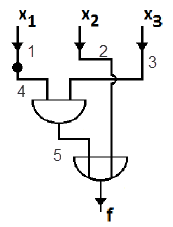
\includegraphics[width=3cm]{images/circuit.png} \hspace{1.5cm}
\begin{tabular}{ll}
$f_1,\dots,f_5$ are 0-jams & $f_6,\dots,f_a$ are 1-jams.\\\hline
 $f_1(x_1,x_2,x_3) = \bar 0x_3+x_2 = x_3+x_2$ & $f_6(x_1,x_2,x_3) = \bar 1x_3+x_2 = x_2$ \\
 $f_2(x_1,x_2,x_3) = \bar x_1x_3+0 = \bar x_1x_3$ & $f_7(x_1,x_2,x_3) = \bar x_1x_3+1 = 1$ \\
 $f_3(x_1,x_2,x_3) = \bar x_10+x_2 = x_2$ & $f_8(x_1,x_2,x_3) = \bar x_11+x_2 = \bar x_1+x_2$ \\
 $f_4(x_1,x_2,x_3) =  0x_3+x_2 = x_2$ & $f_9(x_1,x_2,x_3) =  1x_3+x_2 = x_3+x_2$ \\
 $f_5(x_1,x_2,x_3) = 0+x_2 = x_2$ & $f_a(x_1,x_2,x_3) = 1+x_2 = 1$ \\
\end{tabular}

\vspace{1cm}

Ausfalltafel:
\begin{tabular}{|l||lll||l|l|l|l|l|l|l|l|l|l||l|}\hline
\# & $x_1$&$x_2$&$x_3$&$f_1$&$f_2$&$f_3$&$f_4$&$f_5$&$f_6$&$f_7$&$f_8$&$f_9$&$f_a$&$f$ \\\hline\hline
0  & 0&0&0            & 0   & 0   & 0   & 0   & 0   & 0   & 1   & 1   & 0   & 1   & 0  \\
1  & 0&0&1            & 1   & 1   & 0   & 0   & 0   & 0   & 1   & 1   & 1   & 1   & 1  \\
2  & 0&1&0            & 1   & 0   & 1   & 1   & 1   & 1   & 1   & 1   & 1   & 1   & 1  \\
3  & 0&1&1            & 1   & 1   & 1   & 1   & 1   & 1   & 1   & 1   & 1   & 1   & 1  \\
4  & 1&0&0            & 0   & 0   & 0   & 0   & 0   & 0   & 1   & 0   & 0   & 1   & 0  \\
5  & 1&0&1            & 1   & 0   & 0   & 0   & 0   & 0   & 1   & 0   & 1   & 1   & 0  \\
6  & 1&1&0            & 1   & 0   & 1   & 1   & 1   & 1   & 1   & 1   & 1   & 1   & 1  \\
7  & 1&1&1            & 1   & 0   & 1   & 1   & 1   & 1   & 1   & 1   & 1   & 1   & 1  \\\hline
\end{tabular}

$\Longrightarrow f_1=f_9 ; f_2 ; f_3=f_4=f_5=f_6 ; f_7=f_a ; f_8$

Ausfallmatrix:
\begin{tabular}{|l||lll||l|l|l|l|l||l|}\hline
\# & $x_1$&$x_2$&$x_3$&$f_1$&$f_2$&$f_3$&$f_7$&$f_8$&$f$ \\\hline\hline
0  & 0&0&0            & 0   & 0   & 0   & 1   & 1   & 0  \\
1  & 0&0&1            & 1   & 1   & 0   & 1   & 1   & 1  \\
2  & 0&1&0            & 1   & 0   & 1   & 1   & 1   & 1  \\
3  & 0&1&1            & 1   & 1   & 1   & 1   & 1   & 1  \\
4  & 1&0&0            & 0   & 0   & 0   & 1   & 0   & 0  \\
5  & 1&0&1            & 1   & 0   & 0   & 1   & 0   & 0  \\
6  & 1&1&0            & 1   & 0   & 1   & 1   & 1   & 1  \\
7  & 1&1&1            & 1   & 0   & 1   & 1   & 1   & 1  \\\hline
\end{tabular}

Fehlermatrix:
\begin{tabular}{|l||lll||l|l|l|l|l||l|}\hline
\# & $x_1$&$x_2$&$x_3$&$f\nleftrightarrow f_1$&$f\nleftrightarrow f_2$&$f\nleftrightarrow f_3$&$f\nleftrightarrow f_7$&$f\nleftrightarrow f_8$ & Test\\\hline\hline
0  & 0&0&0            & 0   & 0   & 0   & 1   & 1 & $\star$ \\
1  & 0&0&1            & 0   & 0   & 1   & 0   & 0 & $\star$ \\
2  & 0&1&0            & 0   & 1   & 0   & 0   & 0 & $\star$ \\
3  & 0&1&1            & 0   & 0   & 0   & 0   & 0 & \\
4  & 1&0&0            & 0   & 0   & 0   & 1   & 0 & \\
5  & 1&0&1            & 1   & 0   & 0   & 1   & 0 & $\star$ \\
6  & 1&1&0            & 0   & 1   & 0   & 0   & 0 & \\
7  & 1&1&1            & 0   & 1   & 0   & 0   & 0 & \\\hline
\end{tabular}

$\Longrightarrow$ Testvector: $\{(0,0,0),(0,0,1),(0,1,0),(1,0,1)\}$

\FloatBarrier
\section*{Exercise 6.2 (Unshortenable DNF's fail fast)}
Let $f: \mathbb{B}^n \to \mathbb{B}$ be a boolean function in disjunctive form \emph{containing only prime implicants}
\footnote{The original statement is either wrong or conflicting with the definition from the lecture, see the comment after the proof}, that is 
$f = \bigvee_{i \in I} f_i$ with $f_i = \bigwedge_{k \in K_i} \op_k^i(x_k)$ prime implicants, for 
$K_i \in \mathfrak{P}\{1,\dots,n\}$ and $\op_k^i \in \{x \mapsto x, x \mapsto \neg x\}$.
We call a representation $f = \bigvee_{i \in I} f_i$ \emph{shortenable} if there exists
a subset $\tilde I \subsetneq I$ such that $f = \bigvee_{i \in \tilde I} f_i$, otherwise
we call the representation $f = \bigvee_{i \in I} f_i$ \emph{unshortenable}. Now suppose
that a function $f$ with the representation $f = \bigvee_{i \in I} f_i$ is implemented by
a two-layered circuit with $|I|$ AND-gates in the first layer and one OR-gate (with fan-in
$|I|$) in the second layer.

\noindent{\textbf{Claim:}} The following two statements are equivalent:
\begin{itemize}
  \item[(1)] Every broken connection changes the function of the circuit
  \item[(2)] The corresponding representation $f = \bigvee_{i \in I} f_i \neq 0$ is unshortenable
\end{itemize}

\noindent{\textbf{Remark:}} We have to exclude the degenerate case $f=0$, because otherwise the
standard construction yields $0$ AND-gates, one single OR-gate without any inputs, and a wire
between the OR-gate and the output. This wire can be removed without changing the function.
\begin{figure}
  \centering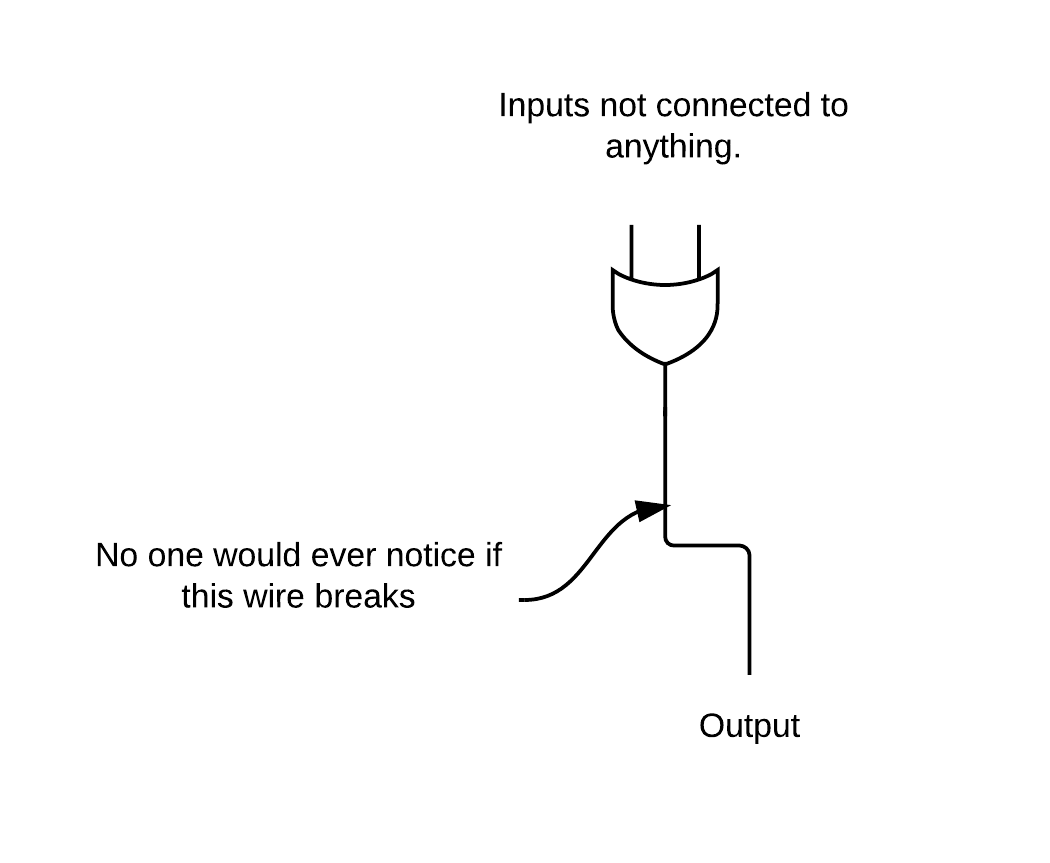
\includegraphics[width=0.4\linewidth]{images/exercise_6_2_degenerate.png}
  \caption{ Degenerate case $f=0$ contains a wire that can break without causing any effects.}
\end{figure}
\FloatBarrier

\noindent{\textbf{Proof:}} We begin with $(1) \Rightarrow (2)$, which is equivalent to
$\neg(2) \Rightarrow \neg(1)$. Suppose the representation $f = \bigvee_{i \in I} f_i$ is
shortenable, that is, there is $\tilde I \subsetneq I$ with 
$f = \bigvee_{i \in \tilde I} f_i$. For each $j \in I \backslash \tilde I \neq \emptyset$ we can destroy
the entire $j-th$ AND-gate together with all the adjacent wires, without changing the 
behaviour of the circuit, in particular, there exists at least one wire that can break without affecting
the circuit. Therefore $\neg (1)$ holds.

To prove $(2) \Rightarrow (1)$ we consider all the possible cases. Let $f = \bigvee_{i \in I} f_i$ be
unshortenable and suppose one connection breaks. Let $\check f$ denote the function implemented by the
broken circuit. Furthermore, let $b_j\in \mathbb{B}^n$ be the boolean vectors such that $m_j(b_j) = 1$
for the $j$-th minterm.

\begin{figure}[h]
  \minipage{0.25\linewidth}
  \centering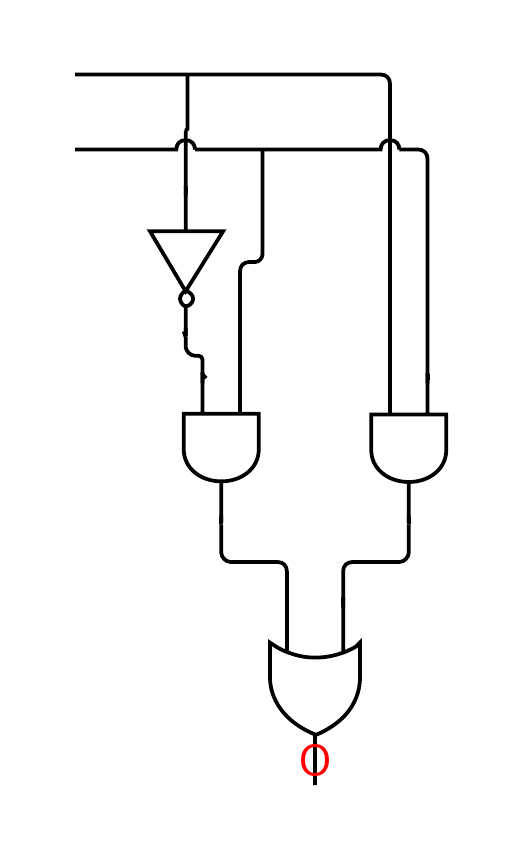
\includegraphics[width=\linewidth]{images/exercise_6_2_output.png}
  \caption{Case 1: \\Broken output wire.}
  \endminipage
  \minipage{0.25\linewidth}
  \centering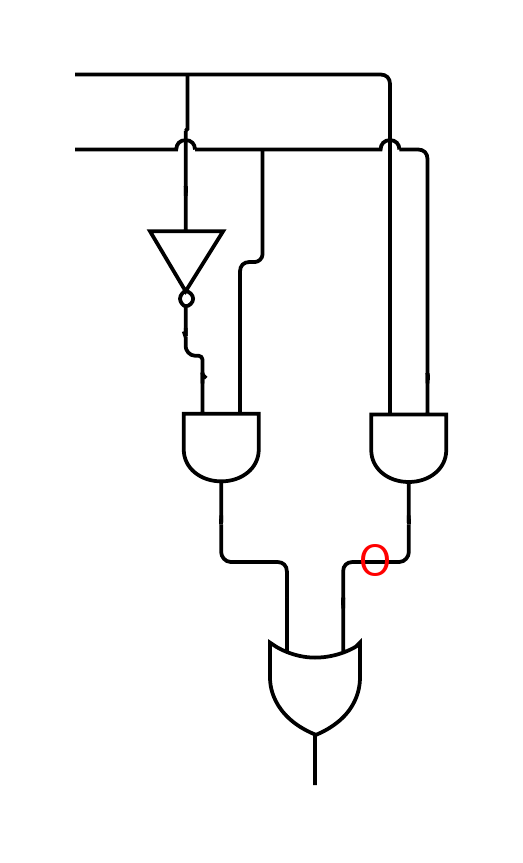
\includegraphics[width=\linewidth]{images/exercise_6_2_and_output.png}
  \caption{Case 2:\\ Broken AND-gate output.}
  \endminipage
  \minipage{0.25\linewidth}
  \centering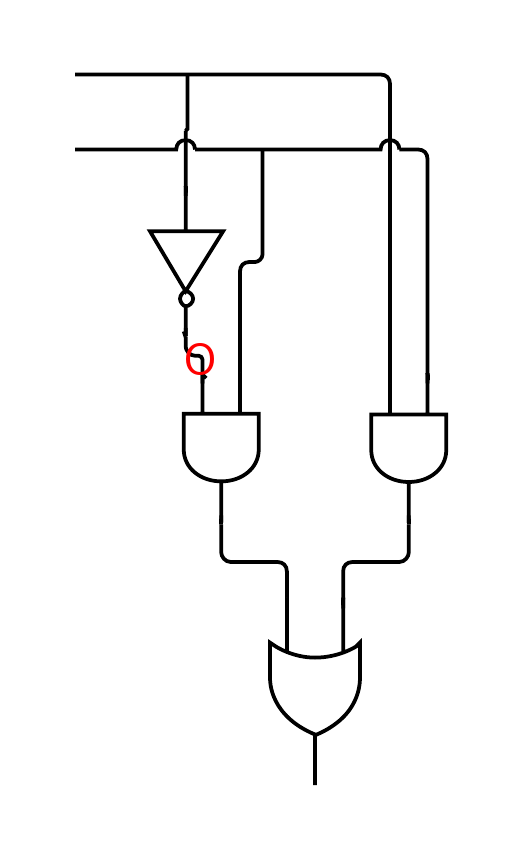
\includegraphics[width=\linewidth]{images/exercise_6_2_after_not.png}
  \caption{Case 3: \\Broken AND-gate input.}
  \endminipage\hfill
  \minipage{0.25\linewidth}
  \centering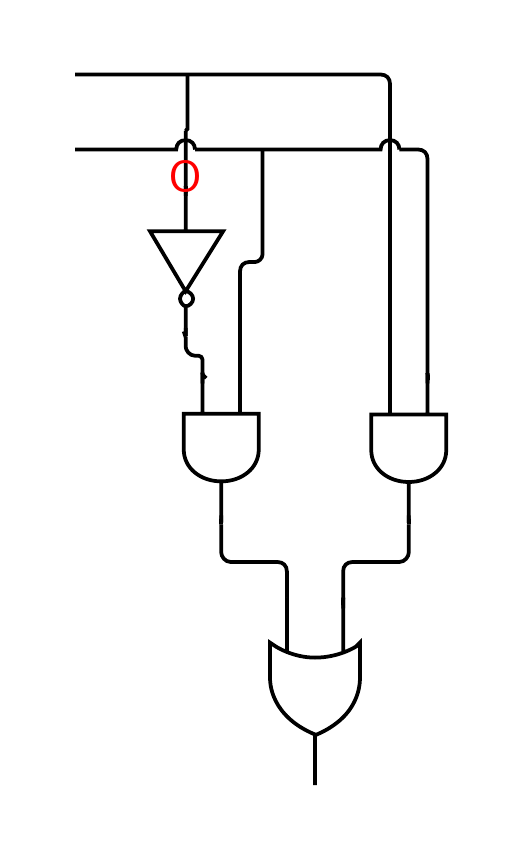
\includegraphics[width=\linewidth]{images/exercise_6_2_before_not.png}
  \caption{Case 4: \\Broken inverter input.}
  \endminipage
\end{figure}

\noindent{\underline{Case 1:}} Suppose the OR-gate output wire breaks. Then $\check f = 0 \neq f$.

\noindent{\underline{Case 2:}} 
Suppose the output wire of an AND-gate breaks. 
If this had no effect on the result, then the conjunction corresponding to this AND-gate 
could be removed from the representation of $f$. This would contradict the assumption that
the representation is unshortenable. Therefore, a broken output of an AND-gate
\emph{has} to affect the circuit.

\FloatBarrier

\noindent{\underline{Case 3:}} 
Suppose an input of an AND-gate breaks (if there is an inverter on the wire, we mean
that the wire breaks right between the inverter and the AND-gate). 
Then one input of the AND-gate is stuck at 0, and the output of the whole 
AND-gate becomes constant $0$, that is, a broken input of an AND-gate has the same 
effect as a broken output in the case 2. Again, this has to affect the whole circuit, 
because otherwise it would contradict the assumption that the representation is
unshortenable.

\noindent{\underline{Case 4:}} 
Finally, suppose that an \emph{input} wire of an inverter breaks. Then one input of the
AND-gate is stuck at 1, and the whole AND-gate behaves as if we removed one variable
from the corresponding term. This has to change the behavior of the whole circuit, 
because otherwise we would get a contradiction to the assumed primality of the term
(we cannot remove variables from prime implicants). \hfill $\blacksquare$

The last case also shows why the original claim is invalid. Consider the circuit used 
in the illustrations as a simple counterexample for the original claim. 
It corresponds to the representation $f = m_1 + m_3 = \bar x y + x y$. It is already in the
normal form, so the minterms are $m_1, m_3$. If we take $m_1, m_3$ as implicants, we 
obtain the implication table:

\vspace{0.5em}
{\centering\begin{tabular}{|c|c|c|}
  \hline
  implicants \textbackslash minterms & $m_1$ & $m_3$ \\
  \hline 
  $\bar x y$ & 1 & 0 \\
  $x y$ & 0 & 1 \\
  \hline
\end{tabular}}
\vspace{0.5em}

Obviously, both rows are required to cover all columns, therefore (according to the
definition given in the solution for the lecture 5) this implication matrix is 
unshortenable. However, breaking the input of the inverter (as on the figure for the
case 4) does not affect the resulting circuit: it still represents just $y = f$. This
is why we had to strengthen the assumption and require that all implicants in the
SOP are prime.

\FloatBarrier
\section*{Exercise 6.3 (Hazards)}

%Dummy table please leave it here

\begin{tabular}{|c||c|c|c|c|}
  \hline
  \multicolumn{5}{|c|}{$x_1=1$} \\ \hline
            & \multicolumn{4}{c|}{$x_4x_5$} \\
$x_2x_3$ & 00                  & 01                  & 11                 & 10                  \\ \hline\hline
    00   &                     & \cellcolor{green}1  &                    &                     \\ \hline
    01   &                     & \cellcolor{green}1  &                    & \cellcolor{magenta}1\\ \hline
    11   & \cellcolor{red}1    & \cellcolor{yellow}1 &                    & \cellcolor{magenta}1\\ \hline
    10   & \cellcolor{red}1    & \cellcolor{yellow}1 &                    &                     \\
  \hline
\end{tabular}\\[5mm]
which yields: $f   =  \textcolor{blue}{\neg x_1x_2\neg x_3\neg x_4}+
                      \textcolor{orange}{\neg x_1\neg x_2\neg x_3\neg x_5}+
                      \neg x_1x_2x_3x_4x_5+
                      \textcolor{red}{x_1x_2\neg x_4}+
                      \textcolor{green}{x_1\neg x_4x_5}+
                      \textcolor{magenta}{x_1x_3x_4\neg x_5}$\\

\end{document}
